\section{Results}
\label{sec:result}
\subsection{Multi-wavelength light curves}
\label{sec:multi-lc}%,fig:x-ray-uv-lc-rp-secondaxis,fig:radio-lc
Multi-wavelength light curves of Mrk~1018 are shown in \autoref{fig:multi-lc-secondaxis}. 
\textcolor{red}{Between 2005 and 2010, the optical/UV flux has started to decline and the X-ray flux is roughly unchanged even Mrk~1018 is in the bright type 1 phase. Between 2010 and 2015, both the optical/UV and X-ray flux shows strong decay in the changing-look phase. A re-flare was found in both optical/UV and X-ray wavebands, where the rise timescale is $\sim 100$ days in X-ray band. During the re-flare,the variation in the optical/UV band is smaller than the variation in X-ray band.} Between 2015 and 2019, the variation is much less in optical/UV band than X-ray band in the fainter type 1.9 phase. After correcting the the radio flux to 5GHz, we find the radio emission roughly keeps unchanged within errors during type I phase and decreases $\sim$ 20 \% after 2015.

We apply the Spearman's rank correlation coefficients to test the correlation between X-ray and optical/UV luminosity in U, UVW1, UVM2 and UVW2 band before and after the changing-look event using the simultaneous \xrt\, and \uvot\, data. We find a positive correlation between the X-ray luminosity ${L_\mathrm{{2-10\,keV}}}$ (${L_\mathrm{{X}}}$) and the optical/UV luminosity ${L_\mathrm{{UV}}}$ during the type 1 and changing-look phase (before MJD 57033), where the Spearman correlation coefficients are 0.99, 0.86, 0.99 and 0.94 ($p$-values are 1.4$\times10^{-24}$, $0.01$, 1.4$\times10^{-24}$ and 4$\times10^{-3}$), respectively. \textcolor{red}{The re-flare deviates the positive correlation.} We do not find an evident correlation between X-ray and optical/UV flux during the type 1.9 AGN phase, where the Spearman correlation coefficients are less than 0.1. 

\begin{figure*}
\centering
	% To include a figure from a file named example.*
	% Allowable file formats are eps or ps if compiling using latex
	% or pdf, png, jpg if compiling using pdflatex
	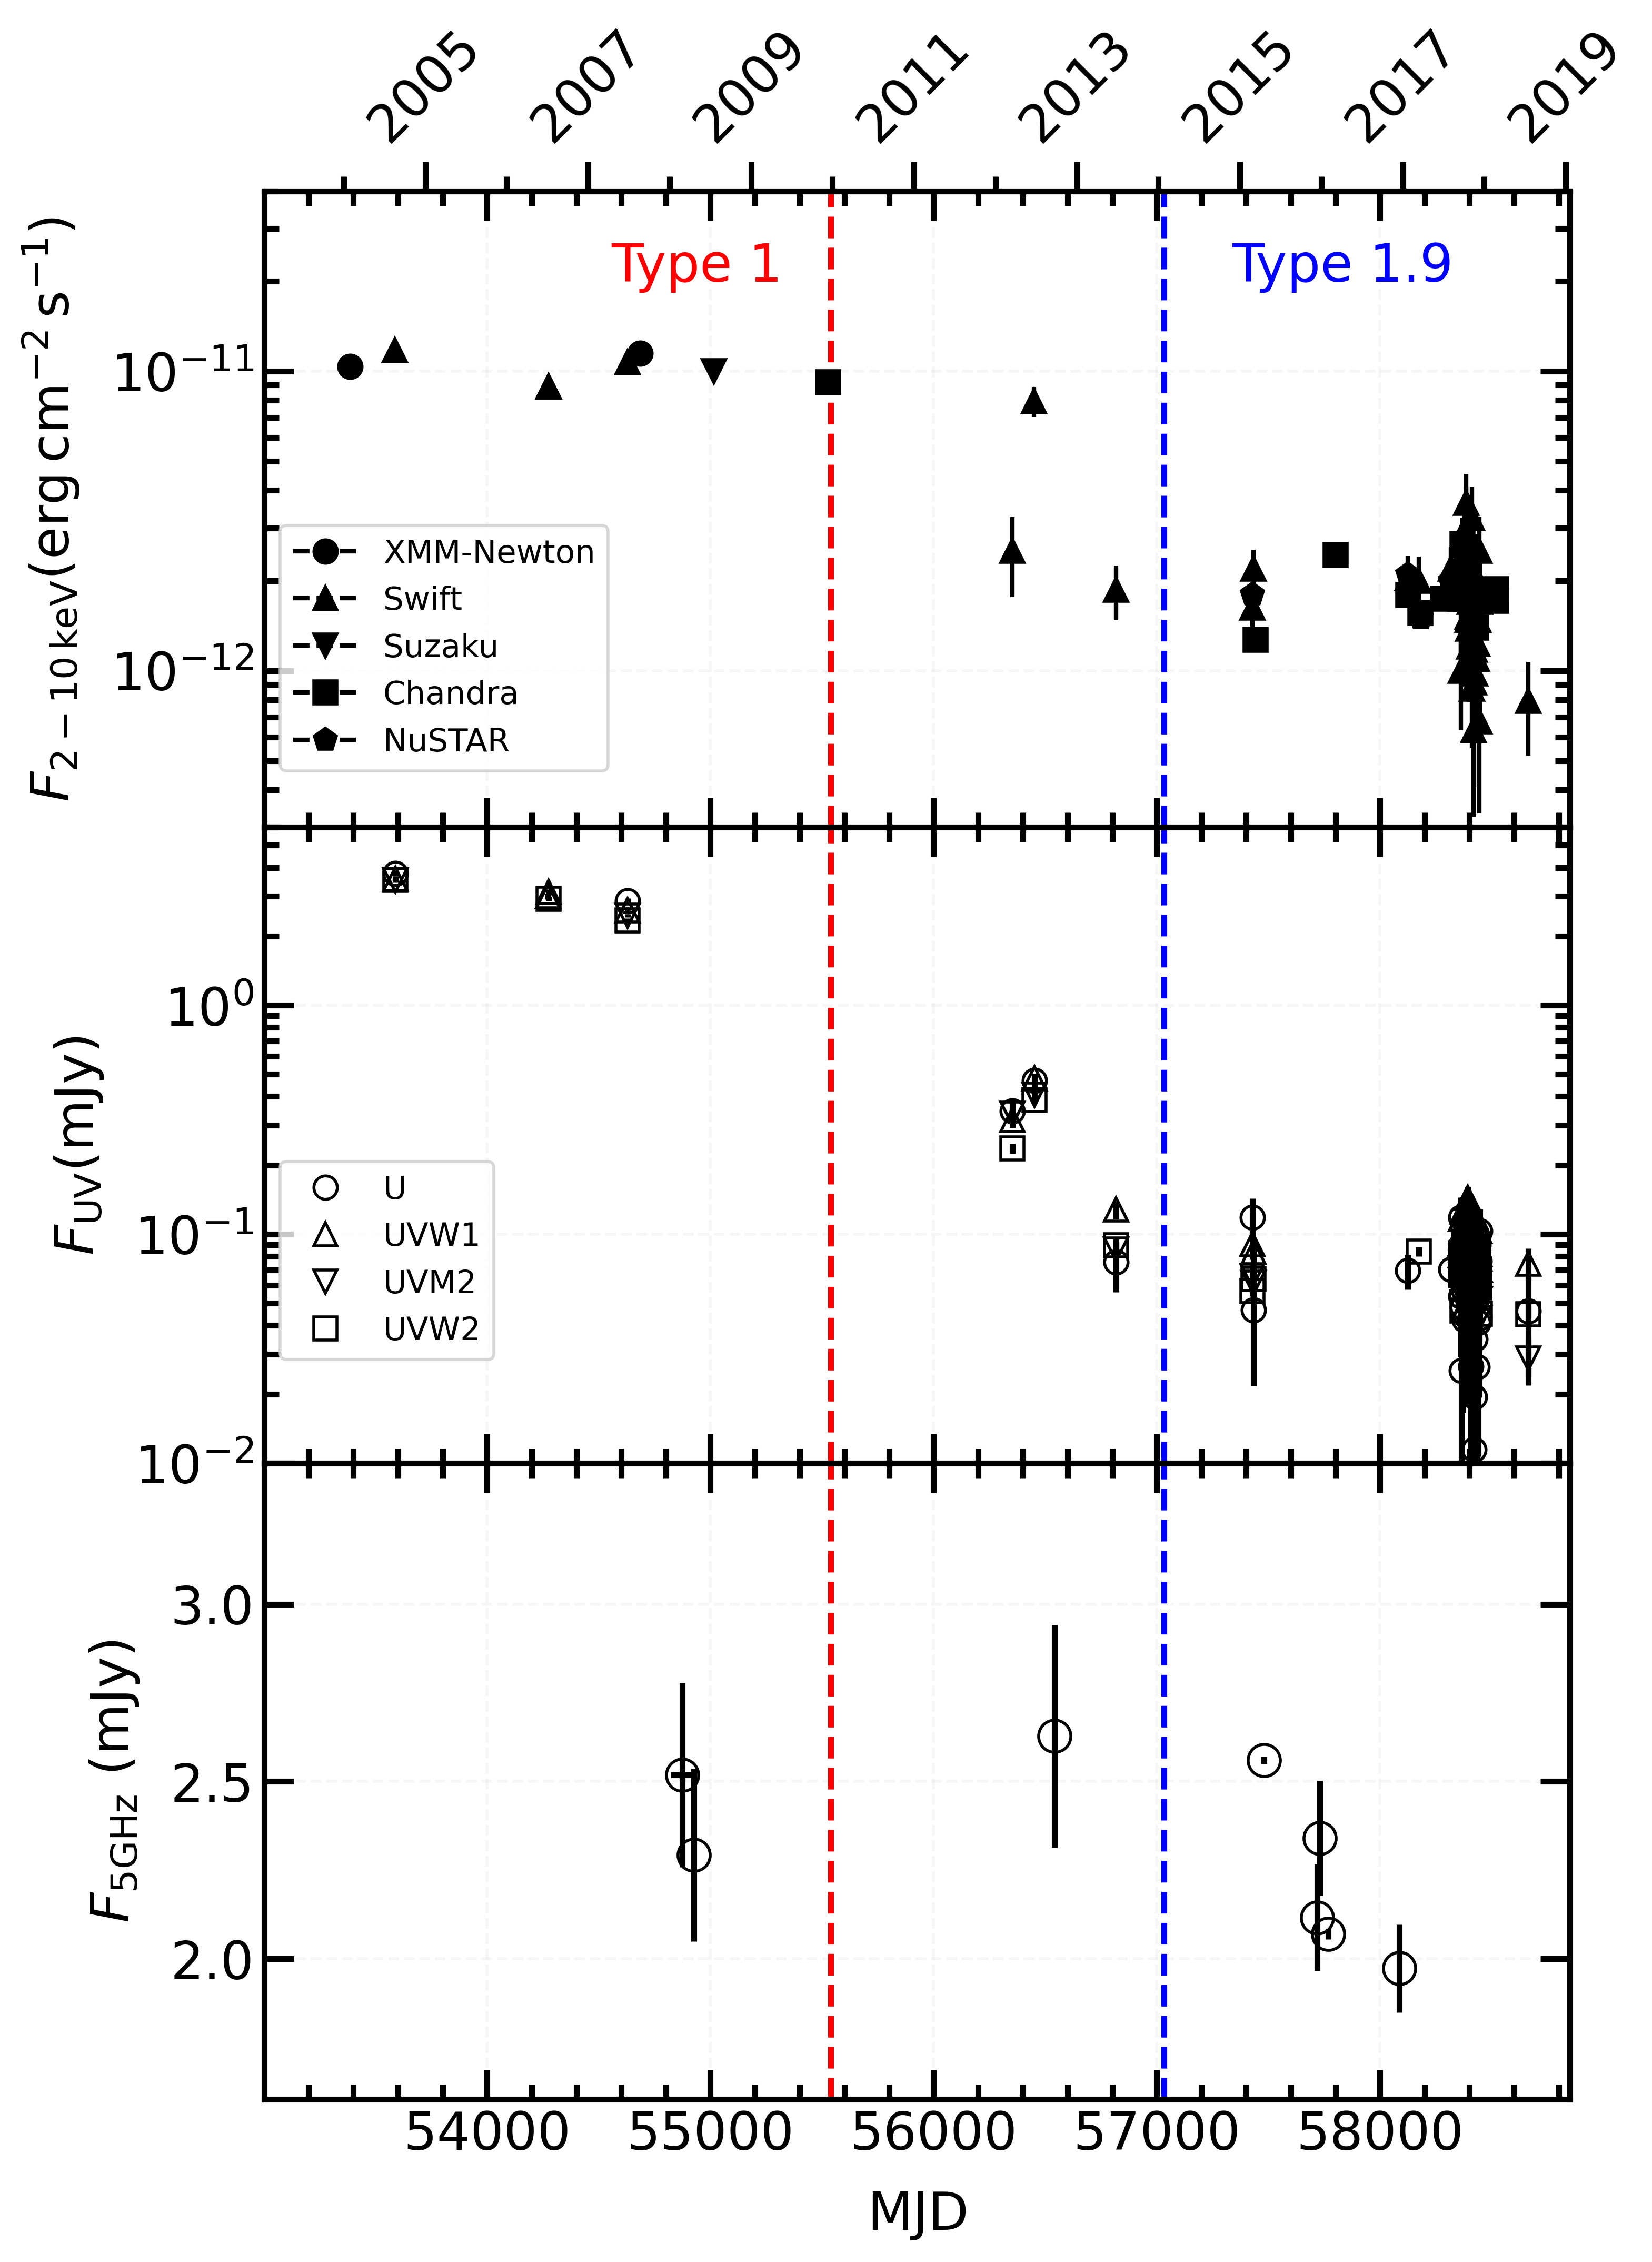
\includegraphics[width=0.9\textwidth]{./pic/subplots-xrt_uvot-radio-second.png}
    \caption{Multi-wavelength light curves of Mrk~1018 between 2005 and 2019. Red and blue vertical dashed lines represent the timeline of optical spectroscopic confirmation at type 1 and type 1.9, respectively. A re-flare during the changing-look phase is found in both the X-ray and the UV bands.}
    \label{fig:multi-lc-secondaxis}
\end{figure*}


  




%\Cref{}
%Radio



\subsection{$\Gamma$-$L_\mathrm{X}/L_\mathrm{Edd}$ and \alphaox- $L_\mathrm{X}/L_\mathrm{Edd}$ correlation}\label{subsec:xray-uv}
The $\Gamma$-$\log{L_\mathrm{X}/L_\mathrm{Edd}}$ correlation can trace the X-ray spectra evolution of AGNs. We present the $\Gamma$-$\log{L_\mathrm{X}/L_\mathrm{Edd}}$ correlation of Mrk~1018 in \autoref{fig:xrayappendgood-Lrateandg-tmap}. Only the data of \xrt\, are presented to avoid the effects of different instruments. We find an evident negative correlation between the photon index ($\Gamma$) and the Eddington-scaled X-ray luminosity ($L_\mathrm{X}/L_\mathrm{Edd}$) in the type 1.9 phase, where we calculated the Spearman correlation coefficient as $-0.6$ ($p$-values is 2$\times10^{-4}$). The data in type 1 phase evidently deviate from the negative correlation. 

%The linear regression of $\Gamma$-$\log{L_\mathrm{X}}$ correlation (parameterised as $\Gamma = k \log{L_\mathrm{X}} +b $ ) yields a slope of $k=-0.87$ in type 1.9. 


The optical/UV-to-X-ray spectral index \alphaox\, is a good indicator of the broad band SED. The \alphaox-$L$ correlation provides useful information on the evolution of the accretion disk and the corona with luminosity in AGNs. $L_\mathrm{2500 \angstrom}$ and $L_\mathrm{2keV}$ are generally used to calculate the \alphaox\, in literatures. We calculate the \alphaox\ with the $L_\mathrm{UVW1}$ from the \uvot\, UVW1 filter with central wavelength {2600{$\angstrom$}} and full-width at half max of $\sim 683\angstrom$ \citep{2008MNRAS.383..627P} and the $L_\mathrm{2keV}$ from X-ray spectra fitting. The host galaxy contribute about half UV emission after 2016 based on the broadband SED modeling from \citet{2018MNRAS.480.3898N}. We subtract the contribution of the host galaxy for $L_\mathrm{UVW1}$ in estimating the \alphaox\,, which is
%\begin{equation}
%\alpha_{OX}  = - \frac{\log(\lambda F_{2600 \angstrom}/\nu F_{2keV})}{\log(\nu_{ 2600 \angstrom }/\nu_{2keV})}+1
%\end{equation}
\begin{equation}
\alpha_\mathrm{OX} = \frac{\log (L_\mathrm{UVW1} / L_\mathrm{2keV} )} {\log (\nu_\mathrm{2keV} /  \nu_\mathrm{UVW1} )}=0.384\times {\log (L_\mathrm{UVW1} / L_\mathrm{2keV} )}
\label{definition_alpha_ox}
\end{equation}
and the $L_\mathrm{2keV}$ from
\begin{eqnarray}
\large{
L_\mathrm{2~keV}= 
\begin{cases}\displaystyle\frac{L_\mathrm{2-10~ keV} (2-\Gamma)}{\nu_\mathrm{2~keV} \times (5^{2-\Gamma}-1)} \quad &, 
\Gamma \neq 2 \\ 
\displaystyle\frac{L_\mathrm{2-10~ keV}}{\nu_\mathrm{2~keV} \times \mathrm{ln} 5}\quad  &, \Gamma = 2
\end{cases} }
\label{definition_f2eV}
\end{eqnarray} 
 We present the \alphaox-$\log{L_\mathrm{X}/L_\mathrm{Edd}}$ correlation in \autoref{fig:alpha_ox_lx}.  We find an evident negative correlation between \alphaox\, and $\log{L_\mathrm{X}}$ in the type 1.9 phase, where the Spearman correlation coefficient is $-0.74$ ($p$-values is 1$\times10^{-6}$).
 
 %The linear regression of \alphaox-$\log{L_\mathrm{X}}$ correlation (parameterised as \alphaox $ = m \log{L_\mathrm{X}} +n$) yields a slope of $m=-0.24$ in type 1.9. 



\begin{figure*}
\centering
	% To include a figure from a file named example.*
	% Allowable file formats are eps or ps if compiling using latex
	% or pdf, png, jpg if compiling using pdflatex
	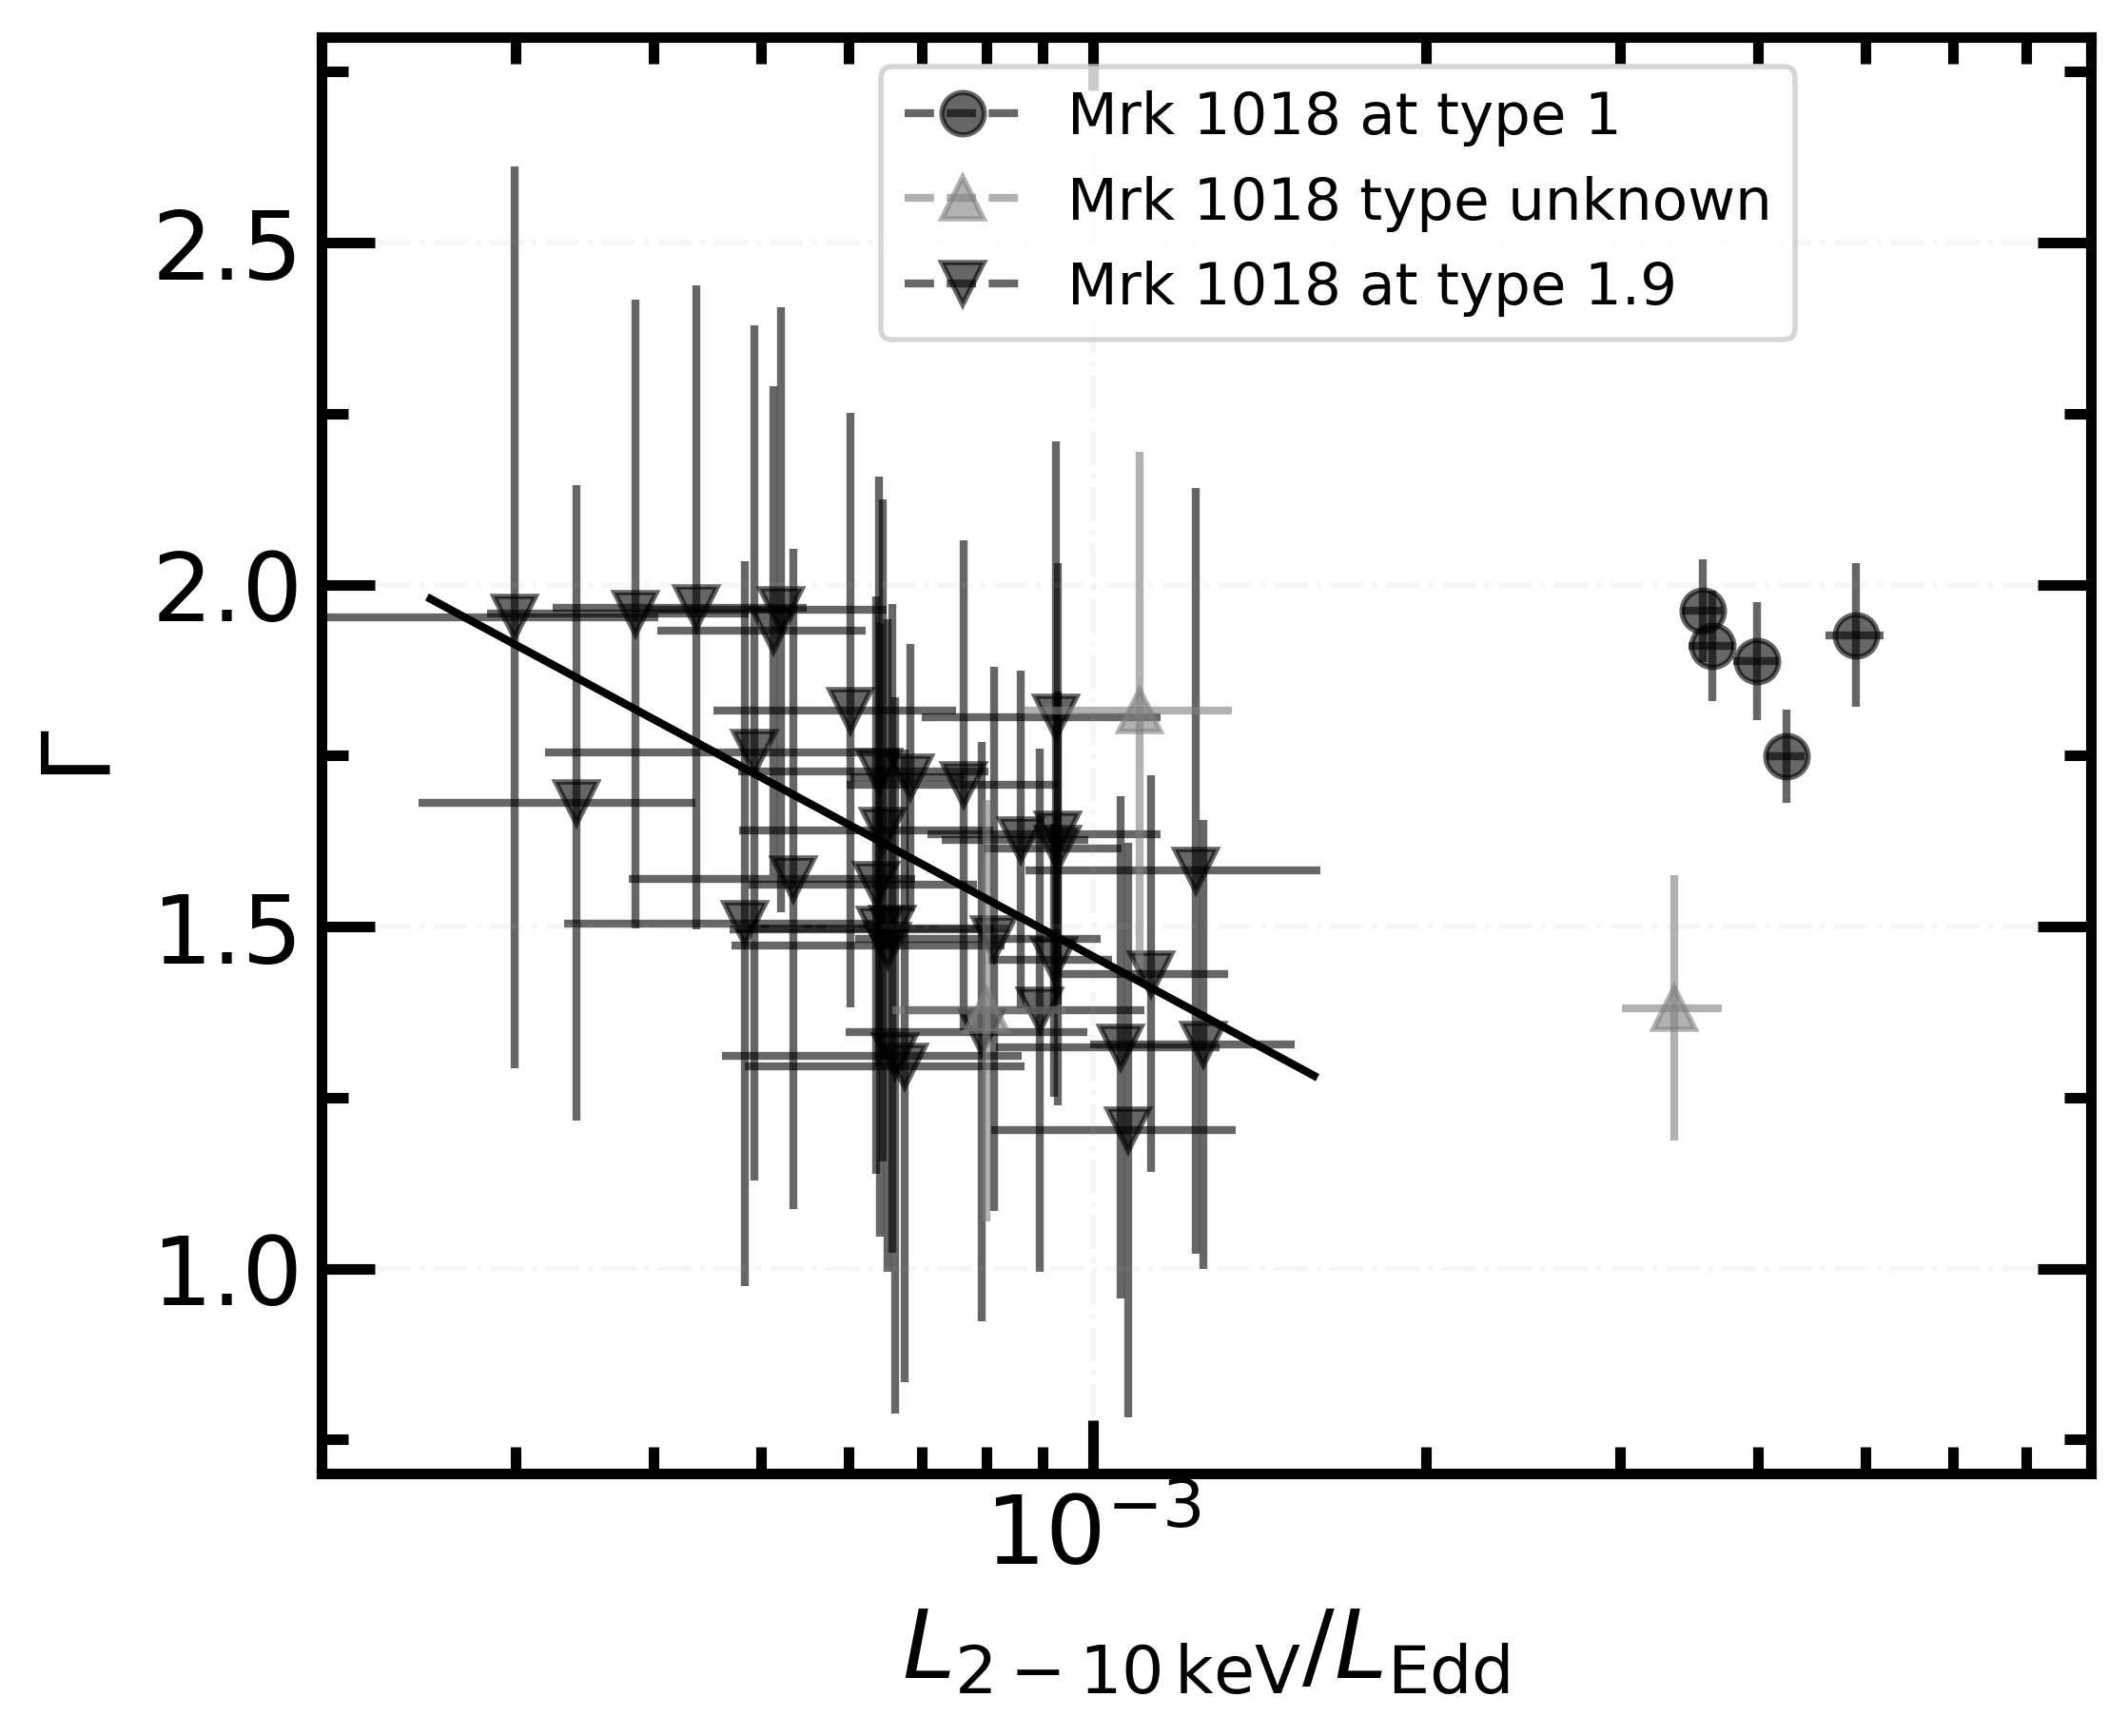
\includegraphics[width=0.65\textwidth]{./pic/xrt_only-errorbar-Lrate-g-tmap_brokenlinear_dot.png}
    \caption{The $\Gamma$ - $L_\mathrm{X}/L_\mathrm{Edd}$ correlation. Only data of \xrt\, are included here. The black solid line represent the best fitting of the negative correlation in the type 1.9.}
    \label{fig:xrayappendgood-Lrateandg-tmap}
\end{figure*}
\begin{figure*}
\centering
	% To include a figure from a file named example.*
	% Allowable file formats are eps or ps if compiling using latex
	% or pdf, png, jpg if compiling using pdflatex
	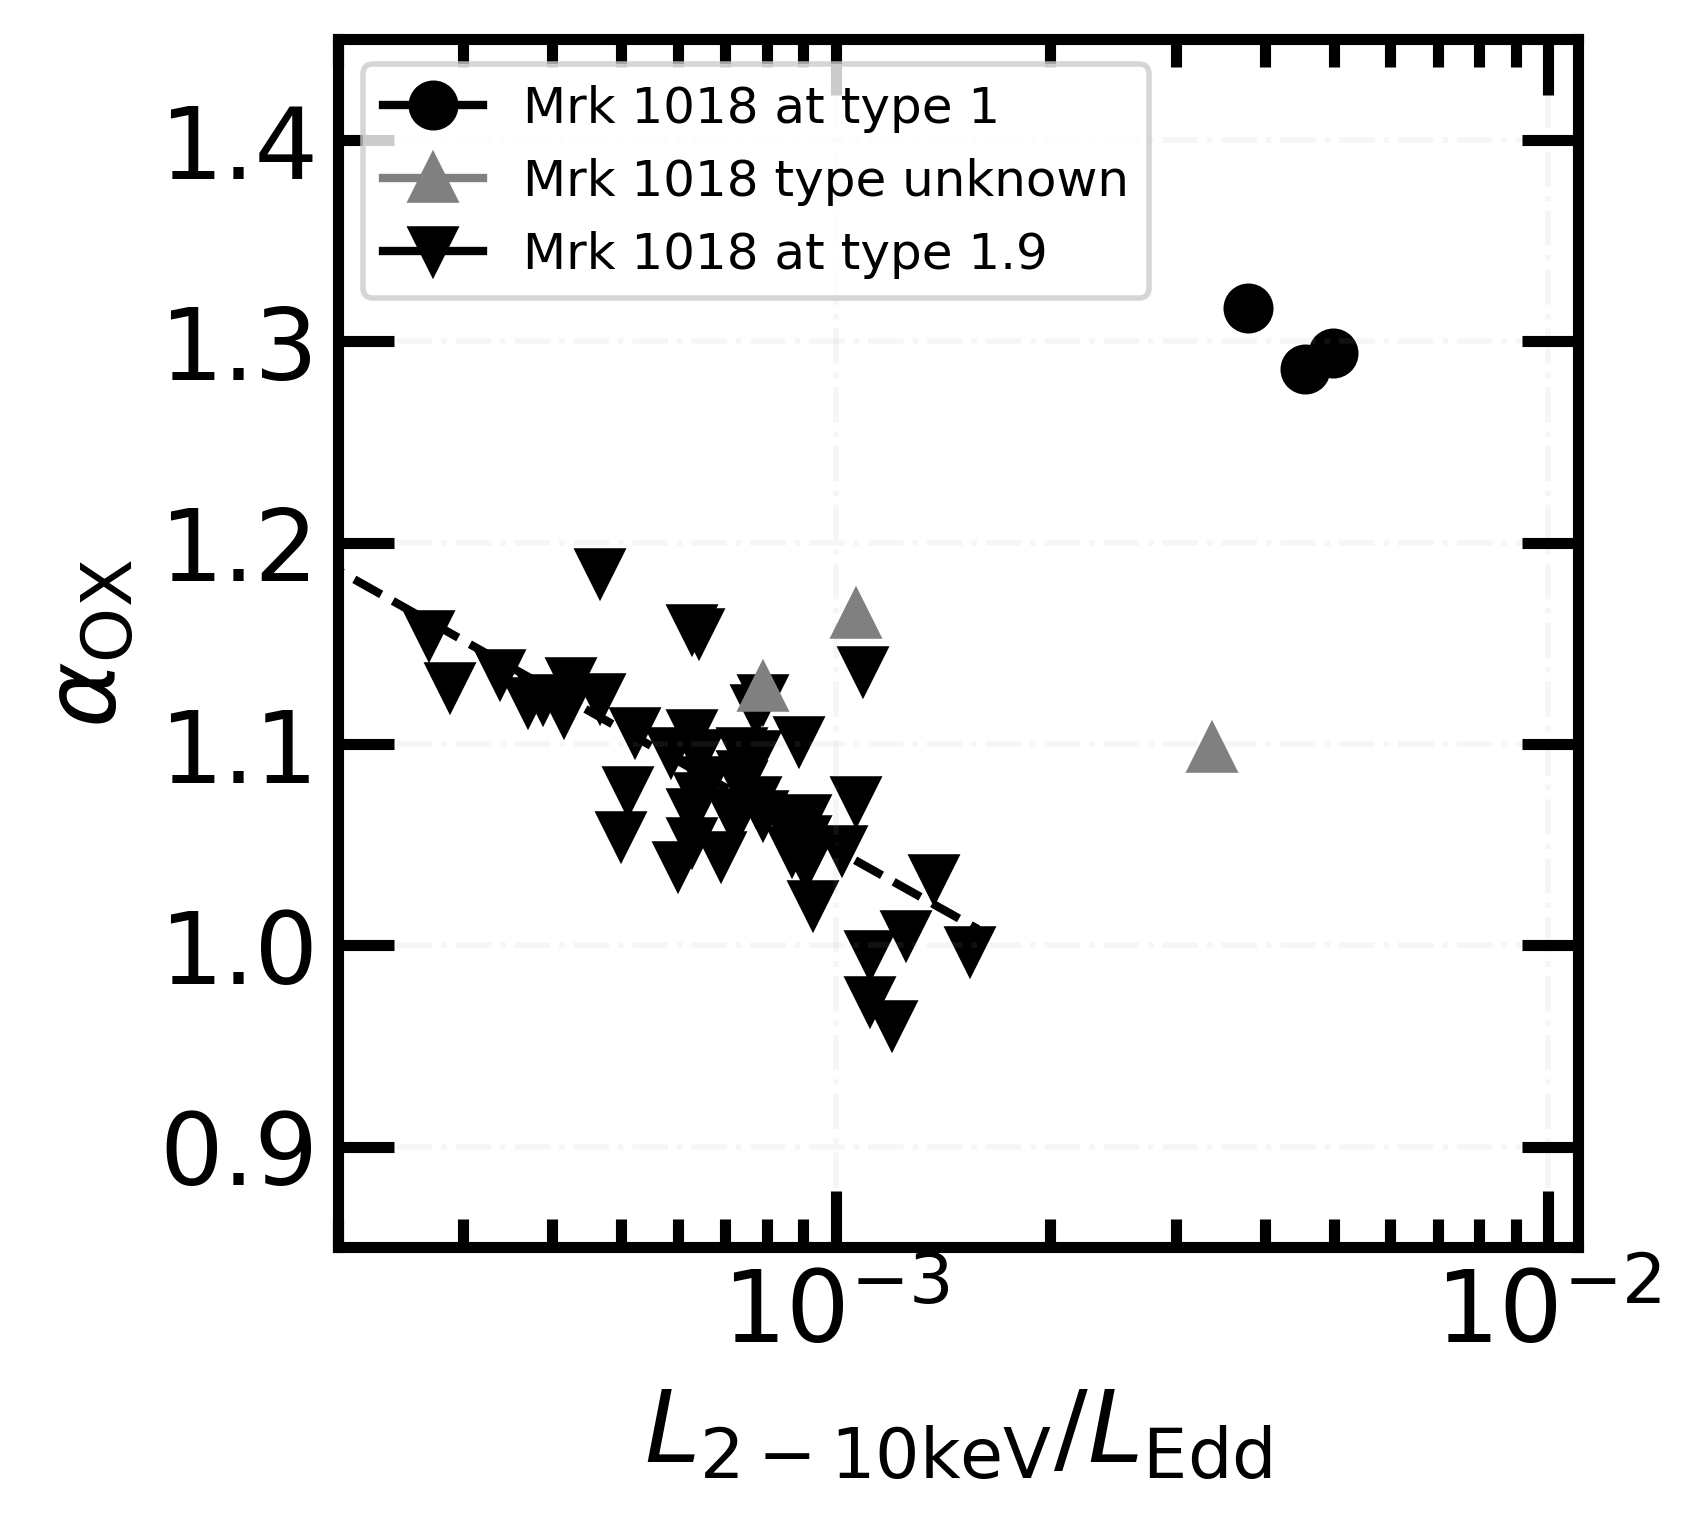
\includegraphics[width=0.65\textwidth]{./pic/Mrk1018_2individuals_alpha_ox_L2-10.png}
    \caption{The $\alpha_\mathrm{OX}-L_{\mathrm{X}}/L_\mathrm{Edd}$ correlation. The black solid line represent the best fitting of the negative correlation in the type 1.9.}   
    \label{fig:alpha_ox_lx}
\end{figure*}


\subsection{Relatively flat R-X correlation}
The radio and X-ray luminosity correlation (R-X correlation hereafter) is a fundamental tool to study the connection between jet and accretion process of black holes. We plot the correlation between the 5 GHz radio luminosity and the nearest X-ray luminosity (interval $\le$ 100 days, see \autoref{tab:radio_xray}) in \autoref{fig:radio-xray-mass_relation_Plotkin2012}. Mrk~1018 roughly follows a flat R-X correlation in the range of $L_\mathrm{X}/L_\mathrm{Edd}$ $\sim$ 3$\times 10^{-4}$-- 4$\times 10^{-3}$.

\begin{figure}
\centering
	% To include a figure from a file named example.*
	% Allowable file formats are eps or ps if compiling using latex
	% or pdf, png, jpg if compiling using pdflatex
	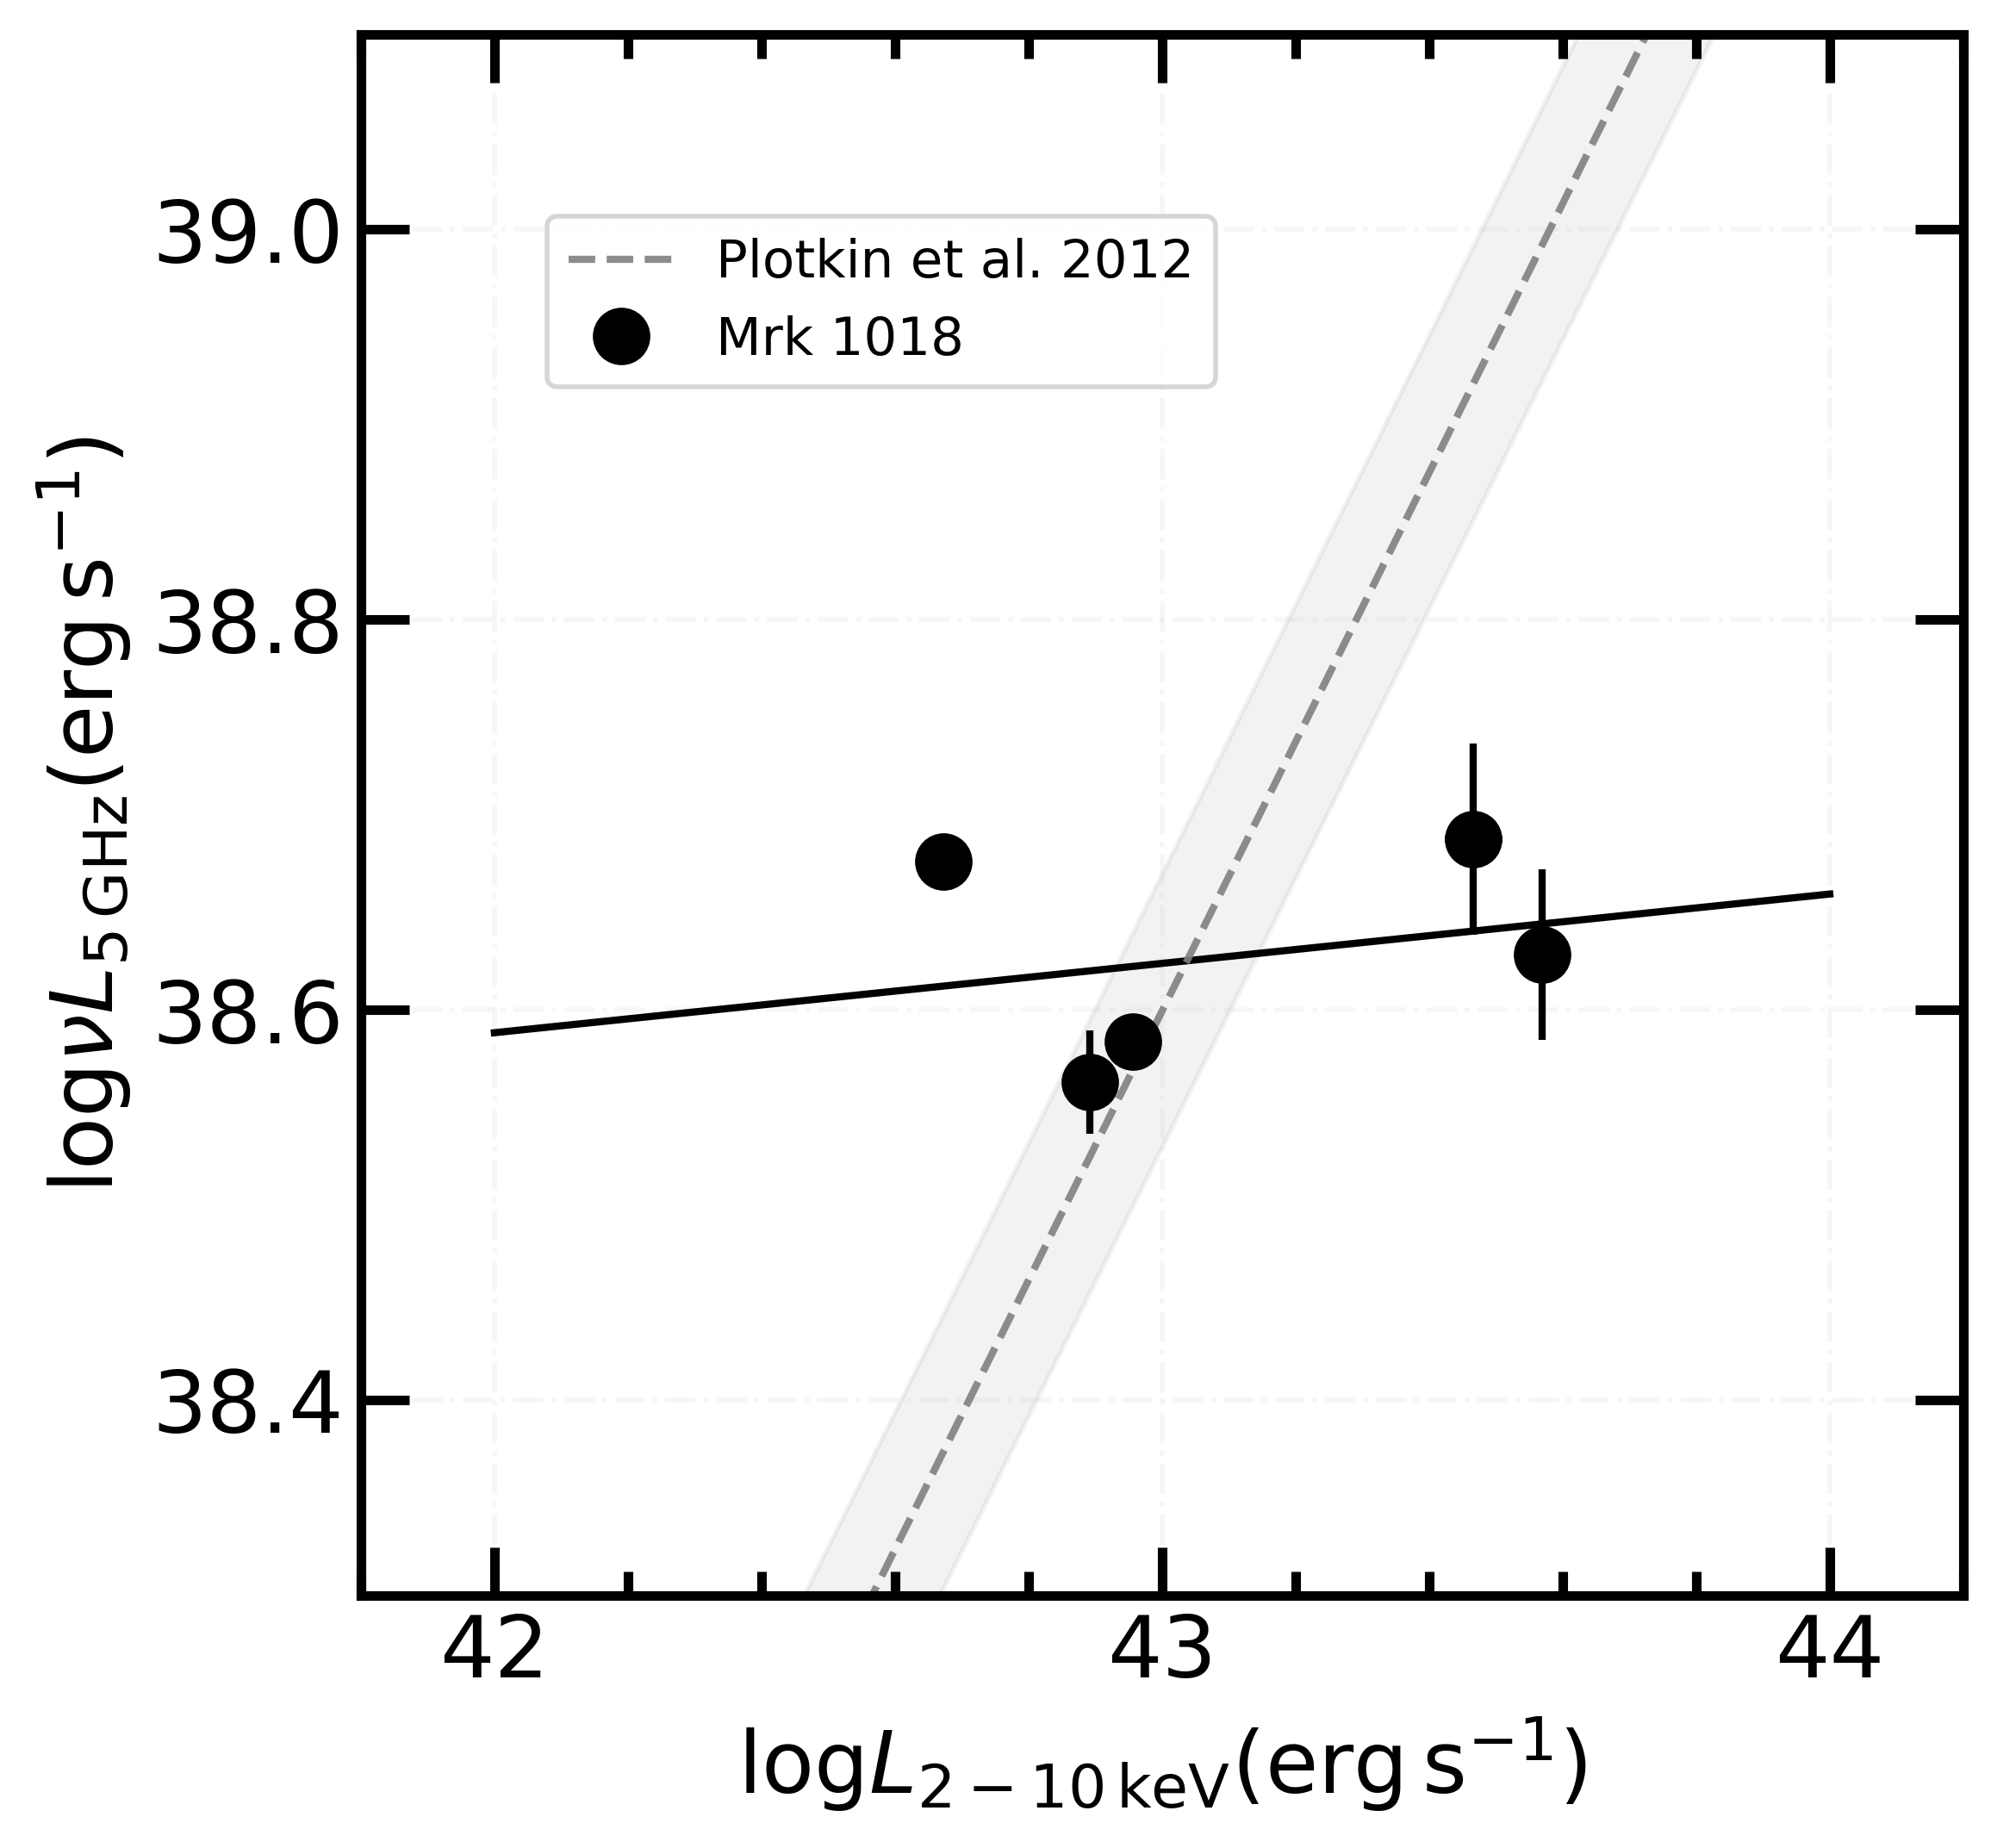
\includegraphics[width=0.45\textwidth]{./pic/Mrk1018_radio_xray_Plotkin2012_Lx.png}
    \caption{The $L_\mathrm{R}$-$L_\mathrm{X}$ relationship. The black solid line shows the best-fitting line of Mrk~1018 with slope of $\sim 0.04$, where the Spearman correlation coefficient is 0.2 ($p$-value is 0.75). The fundamental plane of a sample of black holes in \citet{2012MNRAS.419..267P} is shown in grey dashed line with intrinsic $\sigma=0.07$ for comparison.} 
    \label{fig:radio-xray-mass_relation_Plotkin2012}
\end{figure}